\section*{Introduction}
The detailed spatiotemporal brain dynamics that underlie human perception and cognition are difficult to measure. Invasive techniques with sufficient temporal or spatial resolution, such as depth electrodes or cortical arrays used with epilepsy patients, are only feasible in rare cases and, in addition, do not capture activity from the entire brain.  In comparison, non-invasive measures such as electroencephalography (EEG) and magnetoencephalography (MEG) suffer from poor spatial resolution, and blood oxygen level dependent functional MRI (BOLD fMRI) from poor temporal resolution and indirect coupling to neural activity \cite{Logothetis2008}.  In spite of this, EEG, MEG, and fMRI have been used individually to study functional activity in the human brain, although, by themselves these modalities provide a limited view of the underlying brain dynamics \cite{Alexander2015}.  

Recently, methods enabling simultaneous acquisition of EEG and fMRI (EEG/fMRI) have led to varied analytic approaches aimed at integrating the electrophysiological and hemodynamic information acquired through the simultaneous measurements.  Such approaches offer the potential to provide a more comprehensive picture of global brain dynamics, and will likely offer new insights into how the brain makes rapid decisions  \cite{Huster2012,Jorge2014}. Some of the techniques that have been proposed for combining multi-modal brain signals have separately analyzed the EEG and fMRI data and subsequently juxtaposed the results \cite{Plichta2013,Yuan2010}, while others attempt for a truly integrated approach in order to fully exploit the joint information contained in the data sets \cite{Dahne2015}. In general, simultaneous EEG/fMRI and the associated analysis techniques have been used to identify neuronal sources of EEG trial-to-trial variability, linking them to cognitive processes such as attention \cite{Warbrick2013a} and inhibition \cite{Baumeister2014}. 

\begin{figure}[ht!]
\centering
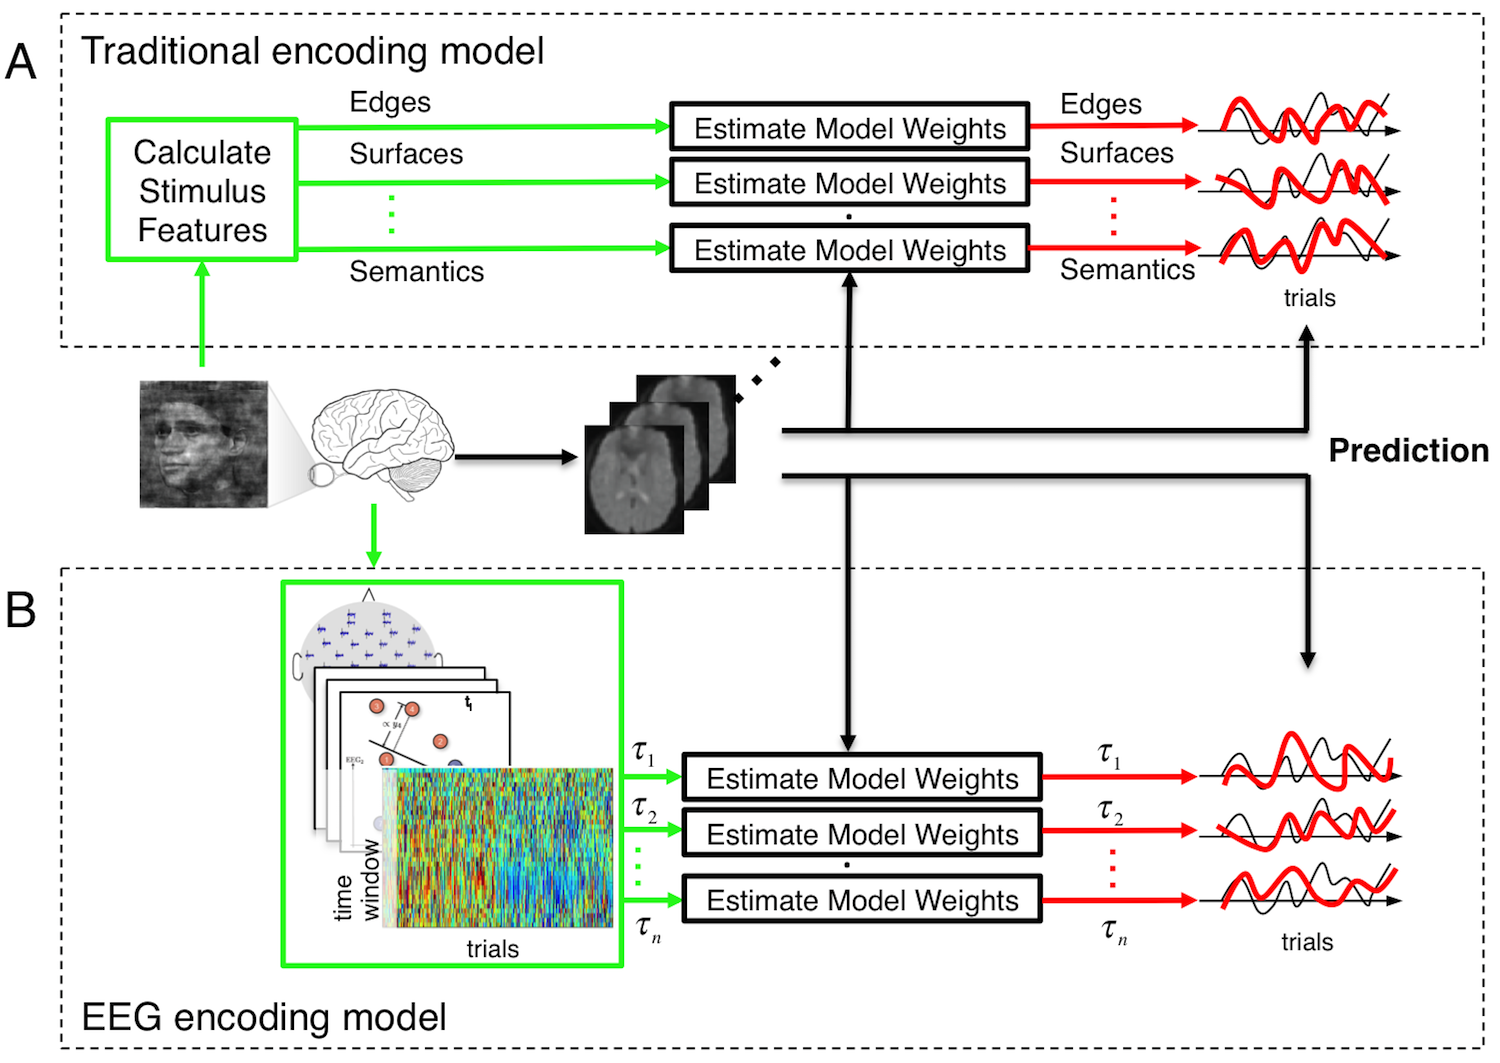
\includegraphics[width=.9\textwidth]{Fig1.png}
\caption{ \textbf{Encoding models based on stimulus derived features versus EEG variability.}\textbf{A}, A traditional encoding model used in fMRI analysis extracts a set of features from the stimulus that are potentially representative of low level structure and high level semantics (green box).  Weights are learned to model how these stimulus features are encoded in the fMRI BOLD signal.  The resulting encoding model is used to make predictions based on how well different voxels predict the features from novel stimuli.  For example, one can create maps of the brain that are labeled based on the stimulus features that each voxel represents. \textbf{B}, The same encoding model concept applied to EEG variability (EEG encoding model).  Instead of features being estimated from the stimulus, they are derived from EEG component trial-to-trial variability (as in Fig 2a) with each temporal window representing a different feature (green box). In traditional encoding models, the stimulus features or concepts are derived through non-linear filters \cite{Cukur2013,Hansen2007,Kay2008,Naselaris2011,Nishimoto2011,Stansbury2013}, however in our model, the non-linearity step is produced by the subject’s brain response to each stimuli which we are able to record with EEG. Weights are learned so as to model how the EEG variability at a given time window is encoded in the fMRI BOLD.  As in the traditional encoding model, predictions on novel stimuli can be done to test the model and results can be used to construct a map —in this case a map of the brain that shows the timing of the EEG component variability that each voxels represents.}
\label{fig:EncodingModel}
\end{figure}

Many previous studies have used known EEG markers (P1, N2, N170, P300, $\alpha$-rhythm) or data driven approaches such as Independent Component Analysis (ICA) to combine EEG with fMRI data \cite{Baumeister2014,DeMartino2010,Huster2012,Jann2009,Jaspers-Fayer2012,Mayhew2013,Nguyen2014,Novitskiy2011,Omata2013,Warbrick2009}. One promising approach has been to use supervised machine-learning techniques (e.g. classifiers) to find relevant projections of the EEG data, where single-trial variability of the electrophysiological response along these projections can be correlated in the fMRI space. Goldman et al.\cite{Goldman2009}, Walz et al.\cite{Walz2013}, Muraskin et al \cite{Muraskin2016}, and Fouragan et al.\cite{Fouragnan2015} have demonstrated this technique on visual and auditory paradigms. This methodology has been shown to localize cortical regions that modulate with the task while preserving the temporal progression of task-relevant neural activity. However, these techniques treat neighboring temporal regions independently when fusing the EEG with fMRI. The approach we present in this paper considers the entire temporal progression of task-specific discriminant activity in the EEG and models how this temporal progression is encoded in the fMRI BOLD data.  Using the full temporal progression allows us to improve temporal resolution and increase the quality of the fit in the encoding model and the accuracy in the subsequent decoding. 

Encoding models have become an important machine learning tool for analysis of fMRI \cite{Naselaris2011}, in that they provide a generative model of the BOLD data (Fig. \ref{fig:EncodingModel}A). In most cases encoding models have been used to learn brain activity that encodes or represents features of a stimulus, such as visual orientation energy in an image/video \cite{Hansen2007,Kay2008,Nishimoto2011}, acoustic spectral power in sound/speech \cite{Silbert2014}, visual imagery during sleep \cite{Horikawa2013} and even high level concepts and semantics \cite{Huth2016}. In the method presented here, however, we employ an encoding model methodology to directly relate the simultaneously collected data from the two neuroimaging modalities. Instead of learning features derived from characteristics of the stimulus, they are derived from the trial-to-trial variability of the EEG components learned via a classifier (Fig. \ref{fig:EncodingModel}B). Specifically, we learn an encoding for the spatially precise fMRI data from the temporally precise trial-to-trial variability of the EEG -- i.e. we learn a mapping that explains the BOLD data given the EEG variability across the time course of each trial. In contrast to previous simultaneous EEG/fMRI techniques that treat the EEG variability at different time points in the trial as independent, we are able to exploit the temporal structure embedded in the EEG by modeling the EEG variability as a time series to accurately predict time course activations in the spatial domain.  

As an example of this method, we apply it to simultaneously acquired EEG/fMRI data collected while subjects performed a perceptual decision-making task. The EEG variability we exploit is derived from a classifier trained to predict the level of stimulus evidence on a trial-to-trial basis from the multichannel EEG data.  This approach leverages the fact that in perceptual decision making tasks, the level of stimulus evidence, as measured via EEG, persists across the trial  \cite{Banko2011a,Philiastides2006}. We can discriminate this information in a time-localized way in the EEG and then temporally ``tag" specific cortical areas by their trial-to-trial variability as they become involved and uninvolved in the decision process. We then proceed to discuss the significance of the results of the new method relative to what can be inferred from non-simultaneously acquired EEG and fMRI.